\section{The Wrapper}


\begin{frame}[fragile]
    \frametitle{Signature to Database Schema}
\begin{columns}
    \begin{column}{0.6\textwidth}
        \vspace{-0.5cm}
        \begin{center}
            schema.sql
        \end{center}
        \vspace{-0.7cm}
\begin{alltt}
CREATE TABLE P(x1 INT, x2 STRING,
               tp INT,
               ts \textcolor{blue}{TIMESTAMP})
               \textcolor{red}{timestamp(ts)};
CREATE TABLE Q(x1 INT, x2 INT,
               tp INT,
               ts \textcolor{blue}{TIMESTAMP})
               \textcolor{red}{timestamp(ts)};
CREATE TABLE R(x1 INT,x2 STRING,
               x3 STRING,
               tp INT,
               ts \textcolor{blue}{TIMESTAMP})
               \textcolor{red}{timestamp(ts)};
CREATE TABLE time_points(tp INT,
                         ts \textcolor{blue}{TIMESTAMP})
                         \textcolor{red}{timestamp(ts)};

\end{alltt}
    \end{column}
    \begin{column}{0.45\textwidth}
        \begin{center}
            signature.sig
        \end{center}
        \vspace{-0.7cm}
\begin{alltt}
P(\textcolor{teal}{id}:int, \textcolor{teal}{action}:string)
Q(\textcolor{teal}{id1}:int, \textcolor{teal}{id2}:int)
R(int, string, string)
\end{alltt}
\vspace{1.1cm}
        
    \end{column}
\end{columns}
\end{frame}

\subsection{Architecture}

\begin{frame}[fragile]{The Wrapper - REST API}
    \begin{columns}
        \begin{column}{0.5\textwidth}
            \begin{itemize}
                \item \texttt{/} (Info-Page)
                \item \texttt{/set-policy}
                \item \texttt{/set-signature}
                \item \texttt{/start-monitor}
                \item \texttt{/stop-monitor}
                \item \texttt{/change-policy}
                \item \texttt{/get-policy} 
                \item \texttt{/get-signature}
                \item \texttt{/reset-everything}
                \item \texttt{/log-events}
                \item \texttt{/get-events}
                \item \texttt{/get-most-recent}
            \end{itemize}
        \end{column}
        \begin{column}{0.5\textwidth}
            \begin{itemize}
                \item \texttt{/db-set-user}
                \item \texttt{/db-set-password}
                \item \texttt{/db-set-host}
                \item \texttt{/db-set-pgsql-port}
                \item \texttt{/db-set-influxdb-port}
                \item \texttt{/db-set-database}
                \item \texttt{/db-get-user}
                \item \texttt{/db-get-password}
                \item \texttt{/db-get-host}
                \item \texttt{/db-get-pgsql-port}
                \item \texttt{/db-get-influxdb-port}
                \item \texttt{/db-get-database}
            \end{itemize}
        \end{column}
    \end{columns}
\end{frame}

\begin{frame}
    \frametitle{The Wrapper - Architecture}
    \centering
    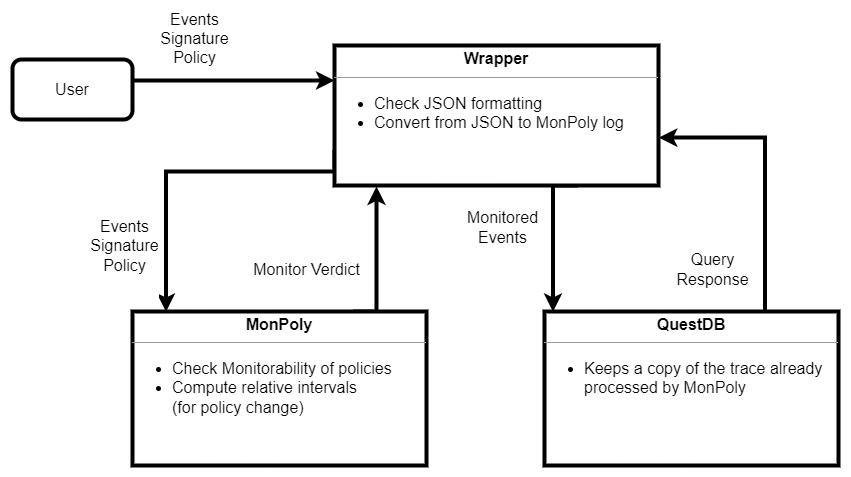
\includegraphics[width=\linewidth]{diagrams/wrapper.png}
\end{frame}

\subsection{The Wrapper - Data flow}

\begin{frame}{Data flow}
    % \centering
    \begin{itemize}
        \item Increased fault tolerance (compared to MonPoly)
    \end{itemize}
    \vspace{1cm}
    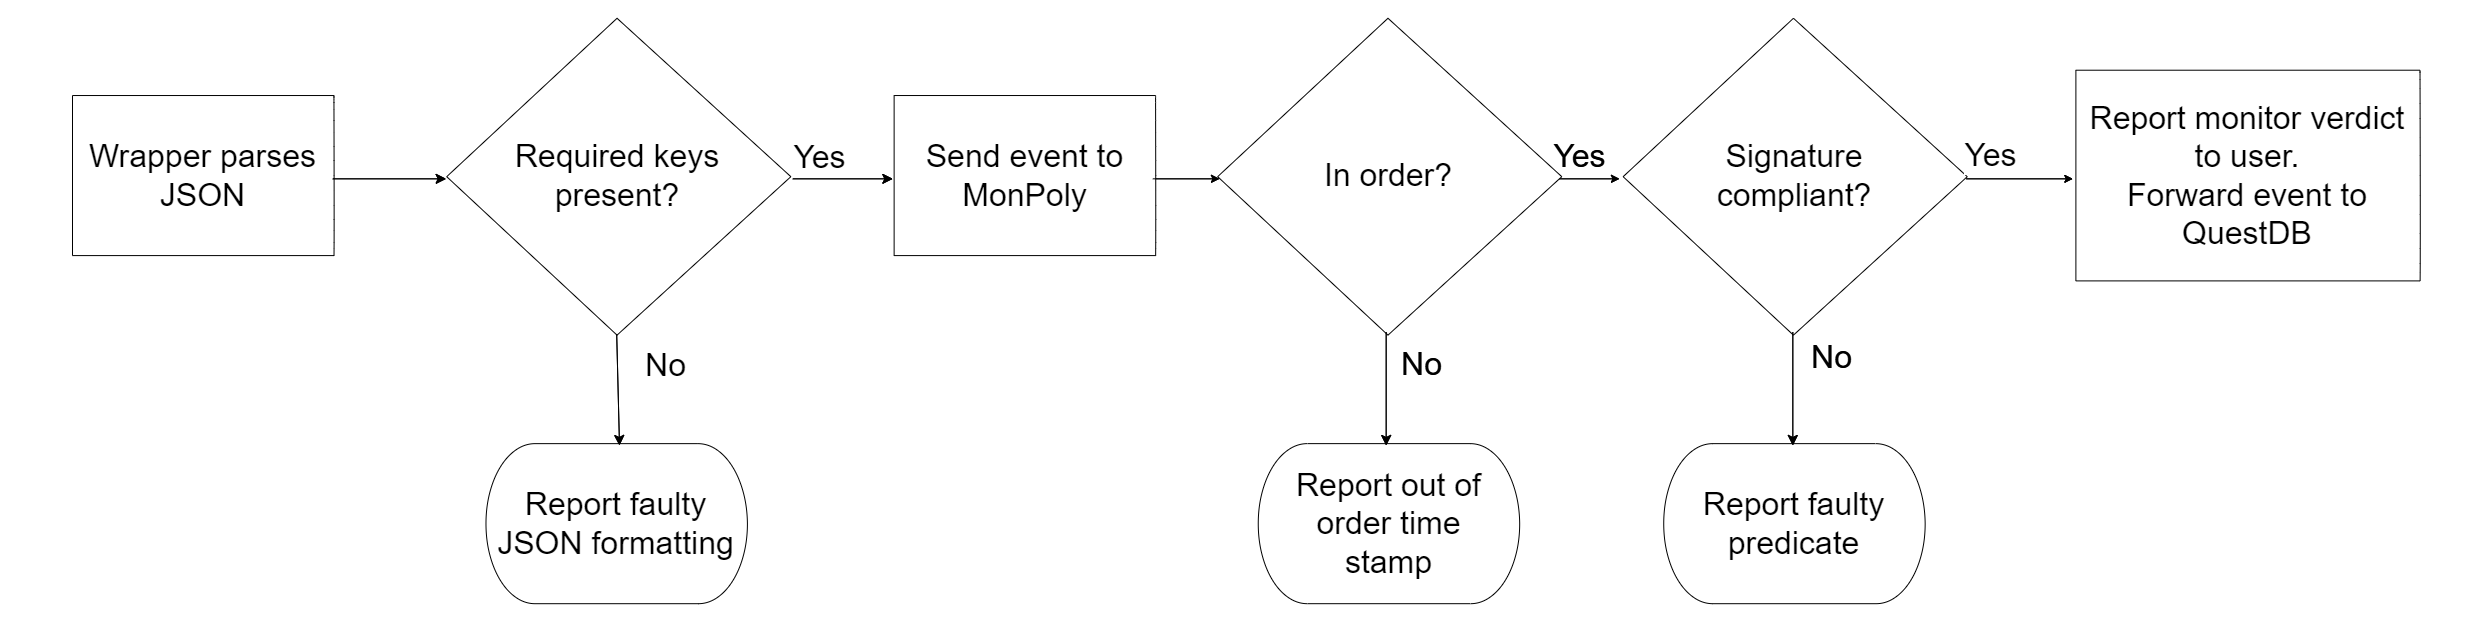
\includegraphics[width=1.0\linewidth]{diagrams/flowchart-2.png}
\end{frame}